\documentclass[12pt, a4paper, openright]{book}

% language
\usepackage[american]{babel}
\usepackage[utf8]{inputenc}

% watermark
\usepackage{draftwatermark}
\SetWatermarkText{DRAFT}
\SetWatermarkScale{4.0}

% bib
\bibliographystyle{plainurl}

% make it look good
\setlength{\parskip}{1.3ex}
\setlength{\parindent}{1.3em}

\usepackage{amsmath}
\usepackage{url}
\usepackage[per=fraction]{siunitx}
%\sisetup{per-mode = symbol}%
\usepackage{listings}

% because the template had it :-)
\usepackage{cite}
\usepackage{fancyhdr}
\usepackage{chngpage}

% I need them :-)
\usepackage[plainpages=false]{hyperref}
\hypersetup {
   pdfauthor={Johannes Wei\ss},
   pdftitle={Multi--Core Energy Accounting},
   pdfsubject={Study Thesis},
   pdfkeywords={multi-core, energy, accounting, Linux}
}
\usepackage{appendix}
\usepackage{longtable}
\usepackage{enumerate}
\usepackage{fancyvrb}
\usepackage{amsfonts}
%\usepackage{geometry}
%\geometry{bindingoffset=1cm}


% KITize it :-)
\usepackage{kitthesiscover}

\newcommand{\JWemail}[1]{\texttt{#1}}
\newcommand{\JWphone}[1]{\texttt{#1}}
\newcommand{\JWemph}[1]{\emph{#1}}
\newcommand{\JWenterprise}[2]{\href{#1}{#2}}
\newcommand{\JWproduct}[2]{\href{#1}{#2}}
\newcommand{\JWlone}[1]{\chapter{#1}}
\newcommand{\JWltwo}[1]{\section{#1}}
\newcommand{\JWlthree}[1]{\subsection{#1}}
\def\TReg{\textsuperscript{\textregistered}}
\def\TCop{\textsuperscript{\textcopyright}}
\def\TTra{\textsuperscript{\texttrademark}}
\def\samples{S}


\title{Multi--Core Energy Accounting}

\begin{document}
\selectlanguage{american}

\frontmatter
%% Titelseite

\title{Multi-Core Energy Accounting}
\author{Johannes Weiß}
\thesistype{sa}
\primaryreviewer{Prof.\ Dr.\ Frank Bellosa}
\secondaryreviewer{Prof.\ Dr.\ Hartmut\ Prautzsch}
\thesisbegindate{15.\ Juni\ 2011}
\thesisenddate{15.\ September 2011}

\maketitle


\tableofcontents

\mainmatter

\cleardoublepage
\JWlone{Introduction}

What is the problem?

Energy is a crucial good especially for mobile devices. Since the energy
available is either limited -- on mobile devices, or can become expensive --
on devices connected to the regular power network, we should use as little as
possible. And since we want to evaluate a whole process, the goal is not to
minimize the instantaneous power but to maximize energy-efficiency.

Even though most modern operating systems try to maximize the CPU utilization
by lowering the frequency \cite{snowdon2010operating} to eventually maximize the
energy-efficiency, this reaction is not always appropriate. A lower CPU
frequency is not always the more energy-efficient
\cite{weissel2002process,snowdon2010operating}.

Thus, for being able to build a good power management, a good power/energy
estimation is critical. The approach used in this study thesis is to use the
CPU's \JWemph{performance counters}.  Since \cite{bellosa2000benefits} there
have been many papers
(\cite{Bertran2010,bertran2010decomposable,kellner03tempcontrol,isci2003runtime,
weissel2002process}, ...) doing energy estimation using performance counters
with really good results.


\begin{itemize}

\item Energy control is important, especially on mobile devices

\item Energy control needs good energy estimation

\item Todays CPUs have many cores and more processes than CPU

\end{itemize}

% vim: set spell spelllang=en_us fileencoding=utf8 :


\JWlone{Technical Prerequisites}
\label{sec:technical-prerequisites}

In this chapter the hardware inspected in this work is presented in detail. The
hardware used to inspect, such as measuring devices, will be depicted in a
chapter of its own (\ref{sec:measuring-device}).

% #  PRODUCTS  #################################################################
\JWltwo{Products}
\label{sec:hw-products}

\begin{itemize}

\item CPU: \JWPcpu (\emph{Sandy Bridge}\cite{wiki:snb} microarchitecture)

\item Mainboard: \JWPboard (unsing an external video controller)

\end{itemize}


% #  SANDY BRIDGE CHARACTERISTICS  #############################################
\JWltwo{Sandy Bridge's Characteristics}
\label{sec:sandy-bridge}

In this section, characteristics of the Sandy Bridge architecture are described
in detail.

\begin{figure}
  \centering
    \includegraphics[width=\textwidth]{fig/intel-cache-orga.png}
  \caption{\JWPcpu cache organization (taken from \cite{intel2011softdev})}
  \label{fig:cache-orga}
\end{figure}


\JWlthree{General}

\begin{itemize}

\item organization: see \ref{fig:cache-orga}

\item L1 cache of \SI{64}{\kibi\byte} per core\cite{intel2011softdev}

\item L2 cache of \SI{256}{\kibi\byte} per core\cite{intel2011softdev}

\item shared L3 cache of \SI{8}{\mebi\byte}\cite{intel2011softdev}

\end{itemize}


\JWlthree{PMU}
\label{sec:sandy-bridge-pmu}

\begin{itemize}

\item ca. 184 events available \cite{intel2011events}

\item 8 general-purpose performance counter registers available per core (4 in
      HT mode) \cite{intel2011softdev}

\item 3 fixed performance counter registers (CPU\_CLK\_UNHALTED, INST\_RETIRED,
      ?) \cite{intel2011softdev,intel2011events}

\end{itemize}


\JWlthree{Architectural Differences between Sandy Bridge and Older Architectures}

Cite \cite{fog11}

\begin{itemize}

\item smaller L2 cache but L3 cache

\item branch prediction

\item pipeline changes

\end{itemize}


\JWlone{Design}
\label{sec:design}

How did I solve the problem?



%#  BIG PICTURE  ###############################################################
\JWltwo{Big Picture of the Setup}
\label{sec:big-pic}

figure and text:

\begin{itemize}

\item Instrumented Sandy Bridge computer counter performance events and is 
      connected to

\item measuring computer which records voltage drops using

\item NI USB-6218.

\end{itemize}

%#  MEASURING SETUP IN DETAIL  #################################################
\JWltwo{Measuring Setup in Detail}
\label{sec:measuring-setup}

In this chapter the measuring setup in detail is presented.


%-  characteristics  -----------------------------------------------------------
\JWlthree{Characteristics}

\begin{itemize}

\item Three differential analog channels: CPU, BOARD, TRIGGER

\item Sampling rate: \SI{50}{\kilo\samples\per\second}

\end{itemize}


%-  wiring scheme  -------------------------------------------------------------
\JWlthree{Wiring Scheme}

In this section a figure of the wiring scheme will be presented. It will contain
every wire, resistor and transistor. It will also include the voltage adjustment
circuit.


%-  measuring device  ----------------------------------------------------------
\JWlthree{Measuring Device}
\label{sec:measuring-device}

For measuring the voltage drops we chose
\JWproduct{http://sine.ni.com/nips/cds/view/p/lang/en/nid/203484}{NI USB-6218}
from \JWenterprise{http://www.ni.com}{National Instruments} because it supports
high sampling rates of up to 250000 samples per second
(\SI{250}{\kilo\samples\per\second}) and is very
accurate (accuracy $< \SI{2.69}{\milli\volt}$)\cite{NISpec2009}.


%#  CALCULATION OF THE ELECTRICAL WORK  ########################################
\JWltwo{Calculation of the Eletrical Work}
\label{sec:calc-work}

From elementary physics

\begin{eqnarray}
     U_R & = & R * I \\
  \iff I & = & \frac{U_R}{R}
\end{eqnarray}

and

\begin{equation}
  U_{CPU} + U_{R} = 12 V
\end{equation}

we obtain the instantaneous power of the CPU by measuring the voltage drop
across the (measuring) resistor:

\begin{eqnarray}
P_{CPU}(t) & = & (12V - U_R(t)) * \frac{U_R(t)}{R} \\
           & = & \frac{12V * U_R - {U_R}^2}{R} \\
           & \stackrel{0 < U_R \ll 1}{\approx} & \frac{12V * U_R}{R}.
\end{eqnarray}

Hence, integrating will result in the electrical work

\begin{equation}
  W = \int P_{CPU}(t)dt.
\end{equation}


%#  THE ENERGY MODEL  ##########################################################
\JWltwo{The Energy Model}
\label{sec:model}

In this section the mathematical and formal methods to find a good subset of
events and their coefficients is presented.

%-  the model's properties  ----------------------------------------------------
\JWltwo{The Model's Properties}
\label{sec:model-properties}

In this work, an energy model is considered as a linear formula. A system with
$N$ CPUs/cores which is able to monitor $M$ performance events per core
simultaneously is described here. Additionally to the per-core event counters,
$K$ system-wide event counters make the model up. In the formal description (see
section \ref{sec:model-pratical} for the practical implementation) we assume
four functions providing the actual values:

\begin{itemize}

\item $g(k)$ the global event $k$'s count in the observed period of time

\item $c(n, m)$ the performance event $m$'s count in the observed period of time
      on CPU/core $n$

\item $w_g(k)$ the global event $k$'s weight in \si{\joule}

\item $w_c(n, m)$ the weight of performance event $m$ in \si{\joule} on core
$n$

\end{itemize}

Though, a energy model equates to

\begin{equation}
W = \sum\limits_{k=0}^K g(m) w_g(m) +
\sum\limits_{n=0}^N \sum\limits_{m=0}^M c(n, m) w_c(n,m)
\end{equation}

. The functions $g$ and $c$ contain the system's life data whereas $w_g$ and
$w_c$ can be calculated a priori as done in this work. Obviously the selection
of the events and their respective weights highly depend on the type of
microprocessor.


%-  minimizing the counter set  ------------------------------------------------
\JWlthree{Minimizing the Set of Performance Events}
\label{sec:min-events}

After having seen (section \ref{sec:model-properties}) what exactly makes up a
model, it crucial to find a small and powerful set of performance events we
actually use. It's not practical to take into account all the events the
microprocessor is aware of. Today's processors offer a lot more events then they
have counters to count them at once \cite{intel2011softdev}.

The approach to find a reasonable subset of $N$ events (of $A$ available) used
in this work can be summed up to:

\begin{itemize}

\item Choose $p$ test programs which utilize the CPU differently. The test
programs have to be independent from external events. We consider subsequent
runs of the test programs as equal.

\item Divide the $A$ available events in $g$ disjoint, non-empty sets $E_{1..g}$
of size up to $N$

\item For each set $E_{1..g}$, run all the $p$ test programs and record the
electrical work and the event counters of the set's events

\item The electrical work of each of the runs of a test program should be
roughly equal.

\item Folding all the results, we gain a vector $W_{1..p}$ of the electrical
work a run of each of the test programs consumes. Additionally, we gain a matrix
$C = [c_{1..p,1..N}]$ containing each event counter's value for a run of each of
the test programs.

\end{itemize}

provide because we need to count them simultaneously. 

\begin{itemize}

\item Take all counters,

\item eliminate equal counters,

\item eliminate linear dependent counters,

\item generate the 5 best models of sizes 1..size(counters),

\item eliminate all counters which appear in no model.

\item Perform exhaustive search on the still-living counters.

\end{itemize}


% vim: set spell spelllang=en_us fileencoding=utf8 :


\JWlone{Implementation}

% vim: set spell spelllang=en_us fileencoding=utf8 :


\JWlone{Evaluation}
\label{sec:evaluation}

This chapter evaluates the usefulness, the accuracy and the overhead the energy
model imposes. The model's strengths and weaknesses are pointed out and it is
compared with a simple computing time based model.


% #  ERROR OF ESTIMATION  ######################################################
\JWltwo{Error of Estimation}
\label{sec:error}

\begin{figure}
  \centering
    \includegraphics[width=\textwidth]{fig/hist-models.eps}
  \caption{Histogram of percent error, sophisticated versus simple model}
  \label{fig:err-hist}
\end{figure}

\begin{figure}
  \centering
    \includegraphics[width=\textwidth]{fig/hist-model-15W.eps}
  \caption{Histogram of percent error for \SI{15}{\watt}\textsuperscript{+}--benchmarks}
  \label{fig:err-hist-15}
\end{figure}

\begin{figure}
  \centering
    \includegraphics[width=\textwidth]{fig/Ncpu-bench-errs.eps}
  \caption{Percent error, sophisticated versus simple model}
  \label{fig:errs-ncpu}
\end{figure}

Most of the 3000 benchmark runs mentioned in chapter \ref{sec:benchmarks} and
\ref{sec:final-model} are estimated with an error of 5\% or better as
\emph{model} in figure \ref{fig:err-hist} shows. The bars named
\emph{cpu\_\-time\_\-based} are a comparison to a simple computing time based
model, discussed in a chapter of its own (\ref{sec:time-based}). The overall
worst sample was estimated with an error of about 40\% (see \emph{model} in
figure \ref{fig:errs-ncpu}). The sample is from a special benchmark run where
all four cores were enabled but mostly idle (real average power usage
\SI{8.9}{\watt}, \SI{12.5}{\watt} estimated). This erratic behavior is
explainable by the design of the model: The goal has been to develop a model
which will not produce completely faultily results but focuses on higher power
consumptions. The power consumptions observed were between \SI{6}{\watt} and
\SI{60}{\watt} and the focus has been set on the range above \SI{15}{\watt}.
This decision was motivated by the fact that an operating system will typically
spend little time in ACPI Processor State C0 \cite{ACPI} when
little energy is consumed. But as chapter \ref{sec:restrictions} states, the
energy model worked out in this thesis is valid iff the CPU is in state C0
all along.  Nevertheless, a similar energy model may be evolved with
particular support for low--power CPU usage and the other ACPI Processor States
in mind.

Regarding most of the benchmarks---which consume more than
\SI{15}{\watt} on average---the model's estimation is clearly better. Figure
\ref{fig:err-hist-15} illustrates a percent error classification of the
benchmarks consuming more than \SI{15}{\watt} on average. The
\SI{15}{\watt}\textsuperscript{+}--benchmarks show an average estimation error
of only 5.3\%.


% #  COMPARISON TO SIMPLE TIME BASED MODEL  ####################################
\JWltwo{Comparison to a simple time based Model}
\label{sec:time-based}

As it is still today's standard to use computing time based models, this chapter
will compare the estimations against the more sophisticated energy model
presented here (chapter \ref{sec:final-model}).

The comparison of the overall average energy estimation error shows the benefit
of a reasonable energy model: 5.4\% versus 13.1\% for the simple computing time
based model. Figure \ref{fig:errs-ncpu} illustrates the results, where the final
energy model is listed as \emph{model} in the figures. The computing time based
model was built by using only the event \JWctr{CPU\_CLK\_UNHALTED} and is
referred to in the figures as \emph{cpu\_\-time\_\-model}. It has been fitted
using a linear regression on the same training data as the regular model,
resulting in the formula

\begin{equation}
W = 5.885J * 10^{-9} * \JWctr{CPU\_CLK\_UNHALTED}.
\end{equation}


% #  OVERHEAD IMPLEMENTATION  ##################################################
\JWltwo{Overhead of this Implementation}
\label{sec:overhead}

To evaluate the overhead of this implementation three metrics have been applied:
Running time, average power usage and unhalted CPU clock cycles. To compare the
results the \emph{473.astar} benchmark of the \JWTLspec{} benchmark suite has
been used. Besides a warm--up run every configuration has been executed ten
times. The performance events have been added consecutively in the order they
are listed in appendix \ref{appendix:chosen-events}. Before measuring the costs
of adding a counter, the system has been benchmarked without even setting up
\JWTlibpfm{} (see chapter \ref{sec:standard-software}). In the plots these
configurations are listed as \emph{0} performance events measured. Because the
unhalted CPU clock cycles are measured using the PMU (chapter {\ref{sec:pmu})
and \JWTlibpfm{}, no benchmark could be recorded without even setting up
\JWTlibpfm{}.

\begin{figure}
  \centering
    \includegraphics[width=\textwidth]{fig/ctr-csts-cycles.eps}
  \caption{Counter Costs Cycles}
  \label{fig:ctr-costs-cycles}
\end{figure}

\begin{figure}
  \centering
    \includegraphics[width=\textwidth]{fig/ctr-csts-time.eps}
  \caption{Counter Costs Time}
  \label{fig:ctr-costs-time}
\end{figure}

\begin{figure}
  \centering
    \includegraphics[width=\textwidth]{fig/ctr-csts-power.eps}
  \caption{Counter Costs Power}
  \label{fig:ctr-costs-power}
\end{figure}

As one can see in figures \ref{fig:ctr-costs-cycles} and
\ref{fig:ctr-costs-time}, the number of counted performance events or using the
PMU (see chapter \ref{sec:pmu}) does not seem to correlate to the clock CPU
cycles or the time a process needs to complete. The Pearson product--moment
correlation coefficients (PCCs) \cite{wiki:PCC} are $-0.18$ with respect to the
running time and $-0.12$ to the clock cycles. Considering the average electrical
power there's some correlation (PCC: $0.72$, figure \ref{fig:ctr-costs-power}),
but the absolute value ($<$ \SI{0.3}{\watt}) is negligible.

So, this implementation does not harm the system's performance and its
contribution to the overall energy consumption is negligible.


% vim: set spell spelllang=en_us fileencoding=utf8 : syntax spell toplevel :


\JWlone{Conclusion}

\begin{itemize}

\item What are the achievements? First Sandy Bridge model.

\item Praise me ;-)

\end{itemize}


% #  PROBLEMS  #################################################################
\JWltwo{Problems}
\label{sec:problems}

What are the problems, what has not been looked at?

\begin{itemize}

\item Suboptimal counter selection? (Multi-core: better events)

\item Short processes lead to fugly results?

\item No true multi-threading (processes running simultaneously do not share
resources

\item Big problem classes as in the following sub sections.

\end{itemize}


%-  no advances features  ------------------------------------------------------
\JWlthree{No DVFS, Hyper-Threading, ACPI Processor States, Turbo Mode, Linux
Dynamic Tics}
\label{sec:no-advances-features}

Because of the limited amount of time and the start from scratch of this thesis,
some enery-relevant processor and operating system features have been disabled.
Since all of these either should work with the current model or individually
raise some kind of events, this is not seen as a major drawback of this work.
Future work may certainly be able to flawlessly integrate them into the known
model. In particular the feature which lasted disabled were:

\begin{itemize}

\item Dynamic Frequency and Voltage Scaling \cite{wiki:DVFS}

\item Hyper-Threading \cite{wiki:HT}

\item ACPI Processor States other than C0 \cite{wiki:ACPI}

\item Intel\TReg{} Turbo Boost Technology 2.0 \cite{wiki:IntelTurboBoost}

\end{itemize}


%-  no auxiliary processing units  ---------------------------------------------
\JWlthree{No Auxiliary Processing Units}
\label{sec:no-aux-units}

In addition to the advanced processor and operating system features meantioned
in chapter \ref{sec:no-advanced-features}, all auxiliary processing units could
not be taken into account. The problem with the auxiliary processing units such
as the floating point unit (FPU), MMX\cite{wiki:MMX}, SSE\cite{wiki:SSE} and
AVX\cite{wiki:AVX} is that they are not or not well covered by the CPU's
performance events (see \cite{intel2011events}). So, they act somehow as a
black box not reveiling the work they do internally. That makes it virtually
impossible to count their energy with the current model.



% #  OUTLOOK  ##################################################################
\JWltwo{Outlook}
\label{sec:outlook}

What could be looked at in future? (what's missing?)

See \ref{sec:problems} :-(.


\backmatter

\addcontentsline{toc}{chapter}{Bibliography}
\bibliography{bibliography}

\appendix
\appendixpage
\addappheadtotoc

\renewcommand\thesection{\Alph{section}}

\JWlappendix{Performance Event Selection and Description}
\label{appendix:chosen-events}

This appendix lists all the performance events that form the energy model
presented in this work. The descriptive texts are all taken from
\cite{intel2011events}.

\begin{itemize}

\item \JWctr{CPU\_\-CLK\_\-UNHALTED}
\begin{quotation}
This is an architectural event that counts the number of thread cycles while the
thread is not in a halt state. The thread enters the halt state when it is
running the HLT instruction. The core frequency may change from time to time due
to power or thermal throttling. For this reason, this event may have a changing
ratio with regards to wall clock time.
\end{quotation}

\item \JWctr{INST\_\-RETIRED}
\begin{quotation}

This event counts the number of instructions retired from execution. For
instructions that consist of multiple micro-ops, this event counts the
retirement of the last micro-op of the instruction. Counting continues during
hardware interrupts, traps, and inside interrupt handlers. Notes:
\JWctr{INST\_\-RETIRED.\-ANY} is counted by a designated fixed counter, leaving
the four (eight when Hyper\-threading is disabled) programmable counters
available for other events. \JWctr{INST\_\-RE\-TI\-RED.\-ANY\_\-P} is counted by
a programmable counter and it is an architectural performance event. Counting:
Faulting executions of GETSEC / VM entry / VM Exit / MWait will not count as
retired instructions.

\end{quotation}

\item \JWctr{BR\_\-INST\_\-RETIRED:FAR\_\-BRANCH}
\begin{quotation}
This is a non-precise version (that is, does not use PEBS) of the event that
counts far branch instructions retired.
\end{quotation}

\item \JWctr{DSB2MITE\_\-SWITCHES}
\begin{quotation}
This event counts the number of the Decode Stream Buffer (DSB)-\-to-\-MITE
swit\-ches including all misses because of missing Decode Stream Buffer (DSB)
cache and u-arch forced misses. Note: Invoking MITE requires two or three cycles
delay.
\end{quotation}

\item \JWctr{DSB\_\-FILL:ALL\_\-CANCEL}
\begin{quotation}
This event counts the number of times when a valid Decode Stream Buffer (DSB)
fill has been actually cancelled not because of exceeding the way limit.
Cancelling Decode Stream Buffer (DSB) fill may also result, for example, from
Decode Stream Buffer Queue (DSBQ) snoop hits. This is because the Decode Stream
Buffer (DSB) full hit is guaranteed to delivery from Decode Stream Buffer (DSB).
In the B step a four-bit counter will count the number of cancel operations and
will reverse the priority upon look ing up the same set.
\end{quotation}

\item \JWctr{ILD\_\-STALL:IQ\_\-FULL}
\begin{quotation}
This event counts stall cycles when instructions cannot be written because IQ is
full. Note: If there is no Resource Allocation Table (RAT) stalls, it indicates
the decoders issue.
\end{quotation}

\item \JWctr{L2\_\-RQSTS:PF\_\-HIT}
\begin{quotation}
This event counts the number of requests from the L2 hardware prefetchers that
hit L2 cache. LLC prefetch new types
\end{quotation}

\item \JWctr{LD\_\-BLOCKS:ALL\_\-BLOCK}
\begin{quotation}
Number of cases where any load ends up with a valid block-code written to the
load buffer (including blocks due to Memory Order Buffer (MOB), Data Cache Unit
(DCU), TLB, but load has no DCU miss)
\end{quotation}

\item \JWctr{LD\_\-BLOCKS:DATA\_\-UNKNOWN}
\begin{quotation}
This event counts the number of load operations delayed due to store buffer
blocks, preceding store operations with known addresses but unknown data.
Counting happens according to the final blocking codes. This does not include
inline wakeups.
\end{quotation}

\item \JWctr{UOPS\_\-DISPATCHED:STALL\_\-CYCLES}
\begin{quotation}
This event counts cycles during which no uops were dispatched from the
Reservation Station (RS) per thread.
\end{quotation}

\end{itemize}



\JWlappendix{File Formats}

\JWlsubappendix{Data Point Files}
\label{sec:fmt:datapoints}

For the definition of the Protocol Buffers used, see appendix
\ref{sec:pb:datapoints}. For the definition of the Protocol Buffer's language
see their
\JWnamedlink{http://code.google.com/apis/protocolbuffers/docs/proto.html}{web
site}.

\input{res/dpts}

\JWlsubappendix{Generic Protocol Buffers}
\label{sec:pb:generic}

This file contains generic Protocol Buffers definitions. Its file path is
\JWpath{protos/generic.proto}.
\begin{Verbatim}[baselinestretch=1,fontsize=\scriptsize]
message Timestamp {
    required int64 sec = 1;
    required int64 nsec = 2;
}
\end{Verbatim}



\JWlsubappendix{Data Points Protocol Buffers}
\label{sec:pb:datapoints}

This file contains the Protocol Buffers definition as used by \JWTlibdp{} (see
chapter \ref{sec:datapoint-files} and \ref{sec:special-developments}). Its file
path is \JWpath{protos/measured-data.proto}.
\begin{verbatim}
import "generic.proto";

message MeasuredData {
    required string shot_id = 1;
    required double sampling_rate = 2;
    required uint32 channel_count = 3;
    required bool has_external_data = 4;
    repeated DataSet inline_data = 5;
    repeated string channel_names = 6; //ordered!
}

message DataSet {
    required Timestamp time = 1;
    repeated DataPoints channel_data = 2;
}

message DataPoints {
    repeated double data_points = 1 [packed=true];
    optional uint32 channel_no = 2;
    optional string channel_name = 3;
}
\end{verbatim}


\JWlsubappendix{Performance Event Counter Protocol Buffers}
\label{sec:pb:counter-files}

This file contains the Protocol Buffers definition as used by \JWTdd{},
\JWTbsle{} and \JWTde{} (see chapter \ref{sec:counter-files} and
\ref{sec:special-developments}). Its file path is
\JWpath{protos/perf-counters.proto}.

\input{res/pb-ctrs}


\end{document}
% vim: set spell spelllang=en_us fileencoding=utf8 :
